\begin{figure}
\centering
\begin{tikzpicture}
\node [anchor=west] (scope) at (-2.5,2.5) {Embodied Costs};
\node [anchor=west] (embodied) at (-2.75,2.0) {(Scope of Chapter)};
\node [anchor=west] (mec) at (-3.1,4.8) {Marginal Cost of Energy};
\node [anchor=west] (bem) at (-3.0,6.8) {Building Energy Model};
\begin{scope}[xshift=1.5cm]
    \node[anchor=south west,inner sep=0] (image) at (0,0) {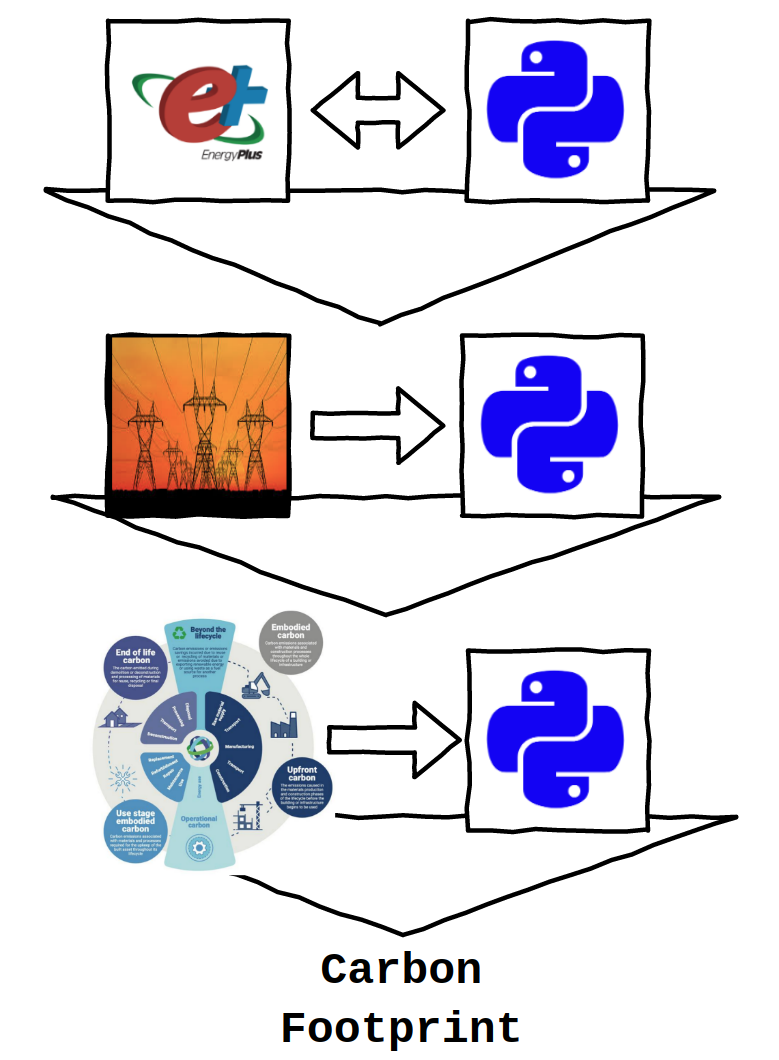
\includegraphics[width=0.4\textwidth]{embodied_cost_model/images/process_flow.png}};
    \begin{scope}[x={(image.south east)},y={(image.north west)}]
        \draw[ultra thick,rounded corners, ,dashed] (1.0,0.45) rectangle (0.0,0.11);
        % \draw [-stealth, line width=5pt, cyan] (scope) -- ++(0.6,0.0);
    \end{scope}
\end{scope}
\end{tikzpicture}
\caption[Model Process Flow Diagram]{Model Process Flow Diagram.}
\label{process_flow}
\end{figure}

c